\documentclass[11pt]{article}
\usepackage{amsmath,textcomp,amssymb,graphicx,comment,tikz}
\usepackage[margin=0.75in]{geometry}
\usetikzlibrary{arrows}
\newcommand{\tab}{\hspace*{2em}}

\def\Name{Alvin Wong (22655478, -cq) , Wai Meng Lei (23985541, -dy) , Chun Yin Yau (24023460, -em)}  % Your name

\title{CS189 --- Homework 7}
\author{\Name}
\markboth{CS189 Homework 7}{CS189 Homework 7}
\pagestyle{myheadings}

\begin{document}
\maketitle
\vspace{5em}
\section*{1. K-Means Clustering on MNIST (page 1 out of 4)}
The code can be run in the code directory, by running the command hw7q1. Note that this may take a while since we use the full 60k MNIST dataset. We initialized the cluster centers to be randomly chosen from the datapoints provided in the training set -- this helps us with preventing clusters with no points. The images for the means are posted below:
\\\\
a) $k = 5$:
\begin{figure}[ht!]
\centering
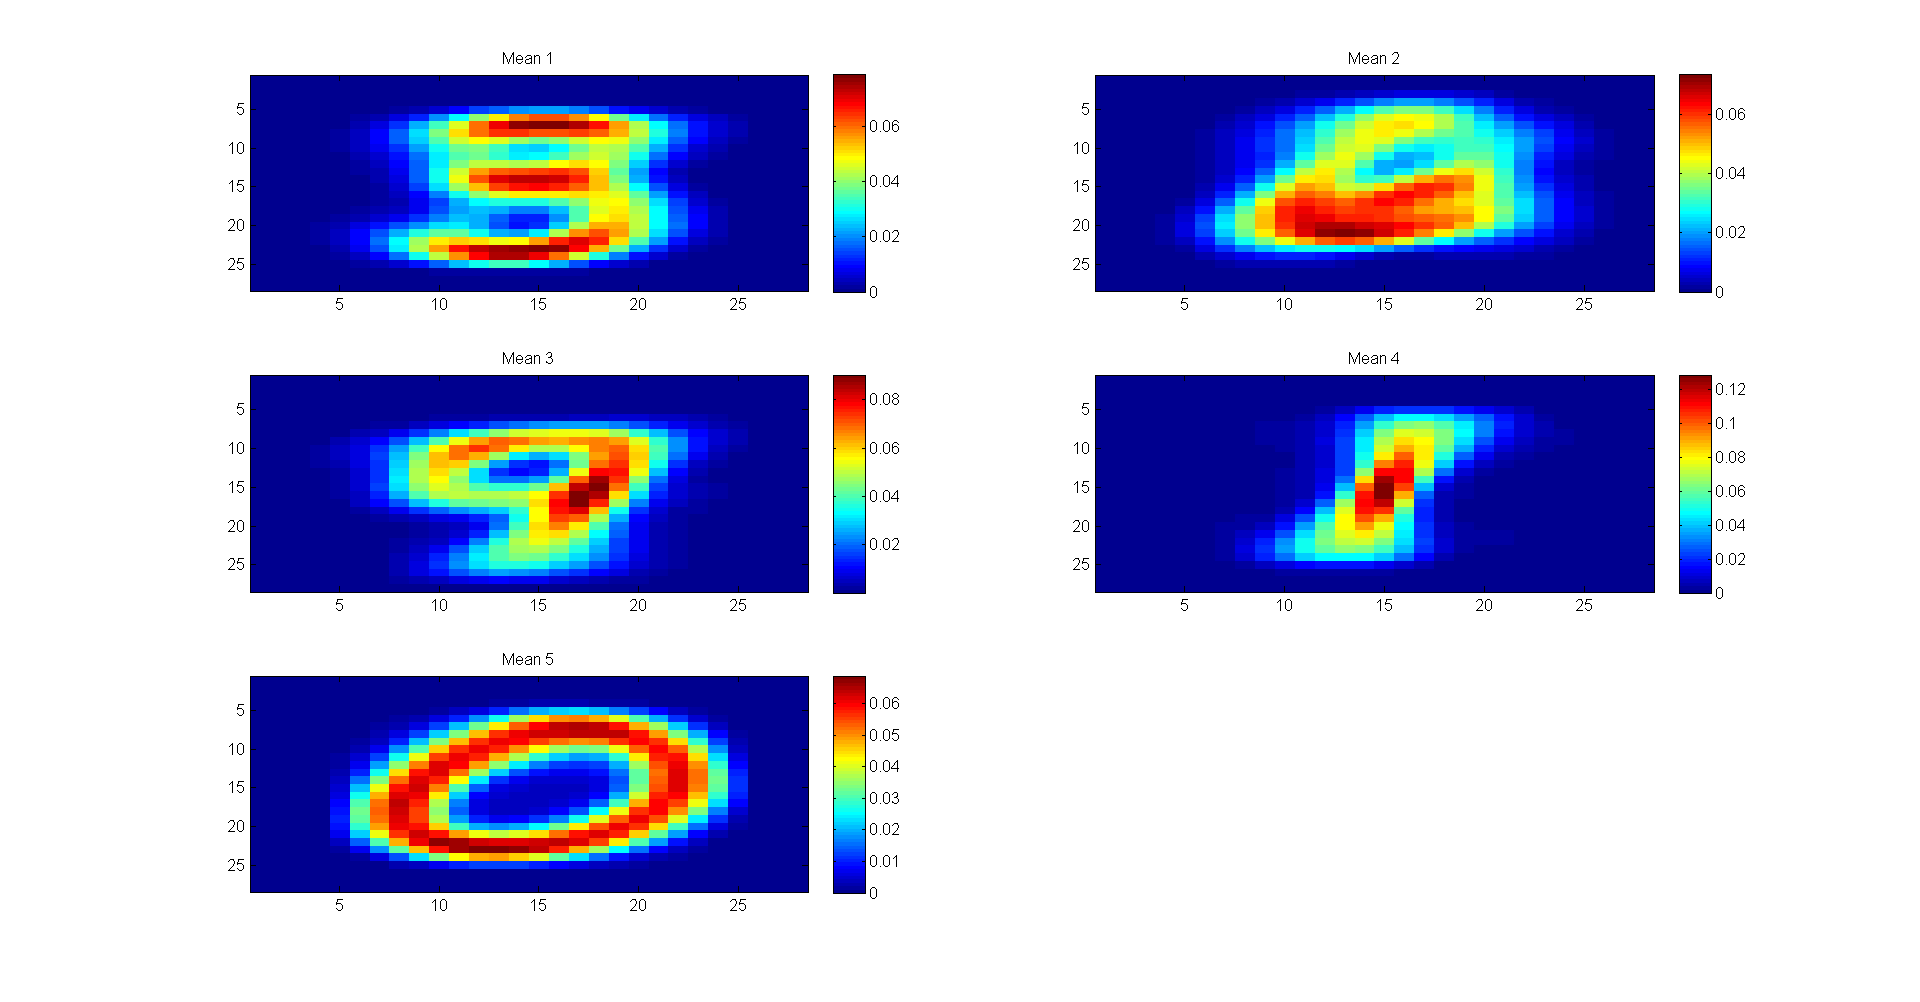
\includegraphics[width=180mm]{images/mean5-1.png}
\label{overflow}
\end{figure}
\newpage
\section*{1. K-Means Clustering on MNIST (page 2 out of 4)}
b) $k=10$:
\begin{figure}[ht!]
\centering
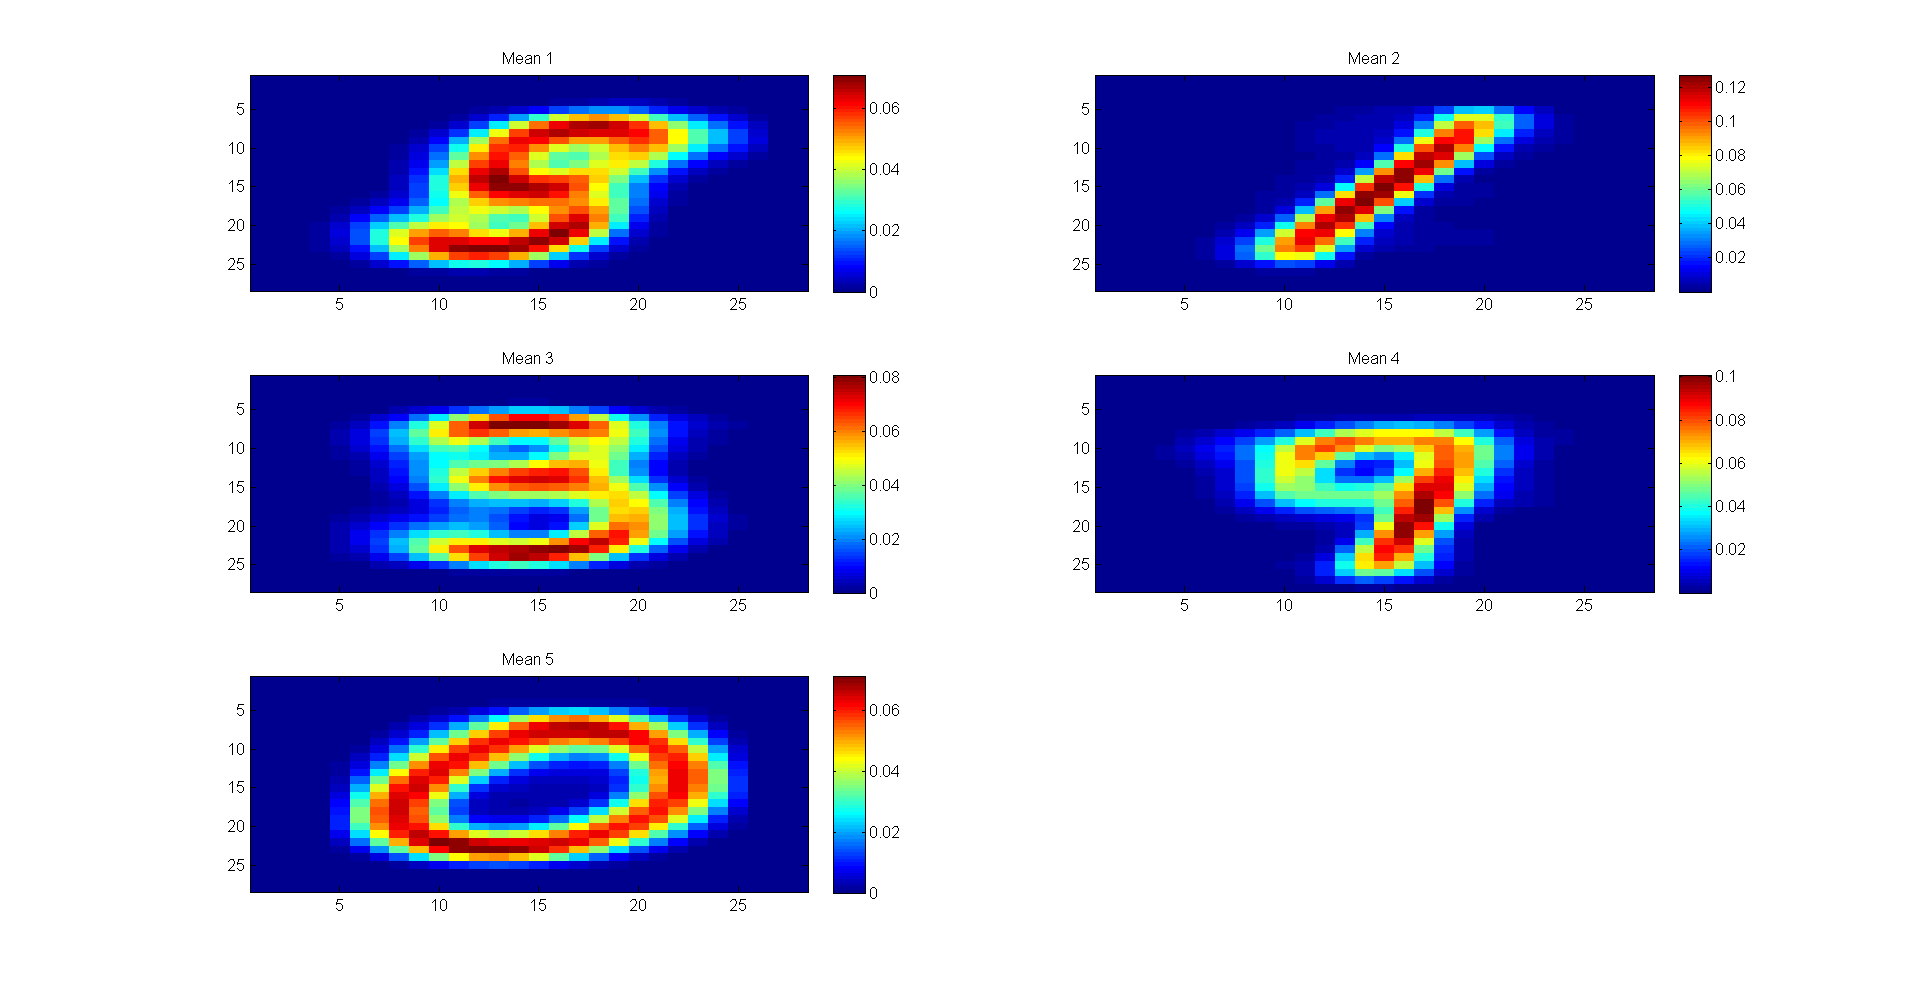
\includegraphics[width=180mm]{images/mean10-1.png}
\label{overflow}
\end{figure}
\begin{figure}[ht!]
\centering
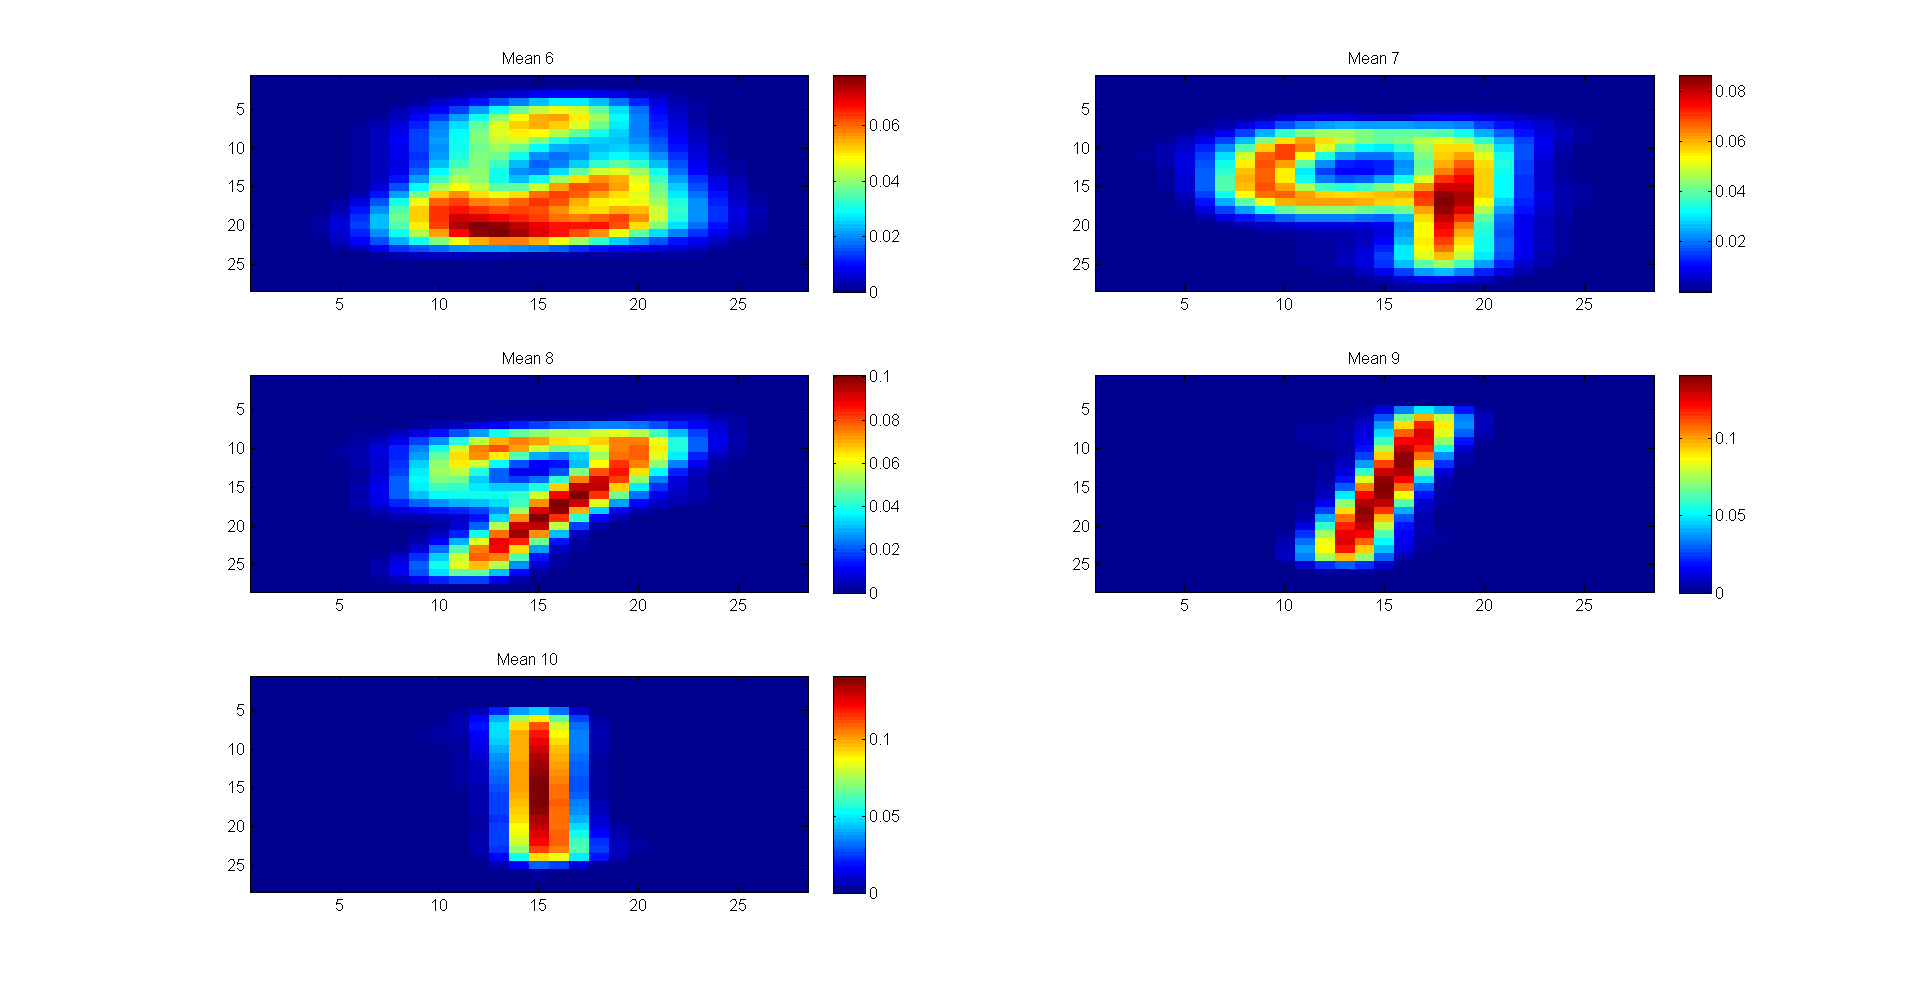
\includegraphics[width=180mm]{images/mean10-2.png}
\label{overflow}
\end{figure}
\newpage
\section*{1. K-Means Clustering on MNIST (page 3 out of 4)}
c) $k=20$:
\begin{figure}[ht!]
\centering
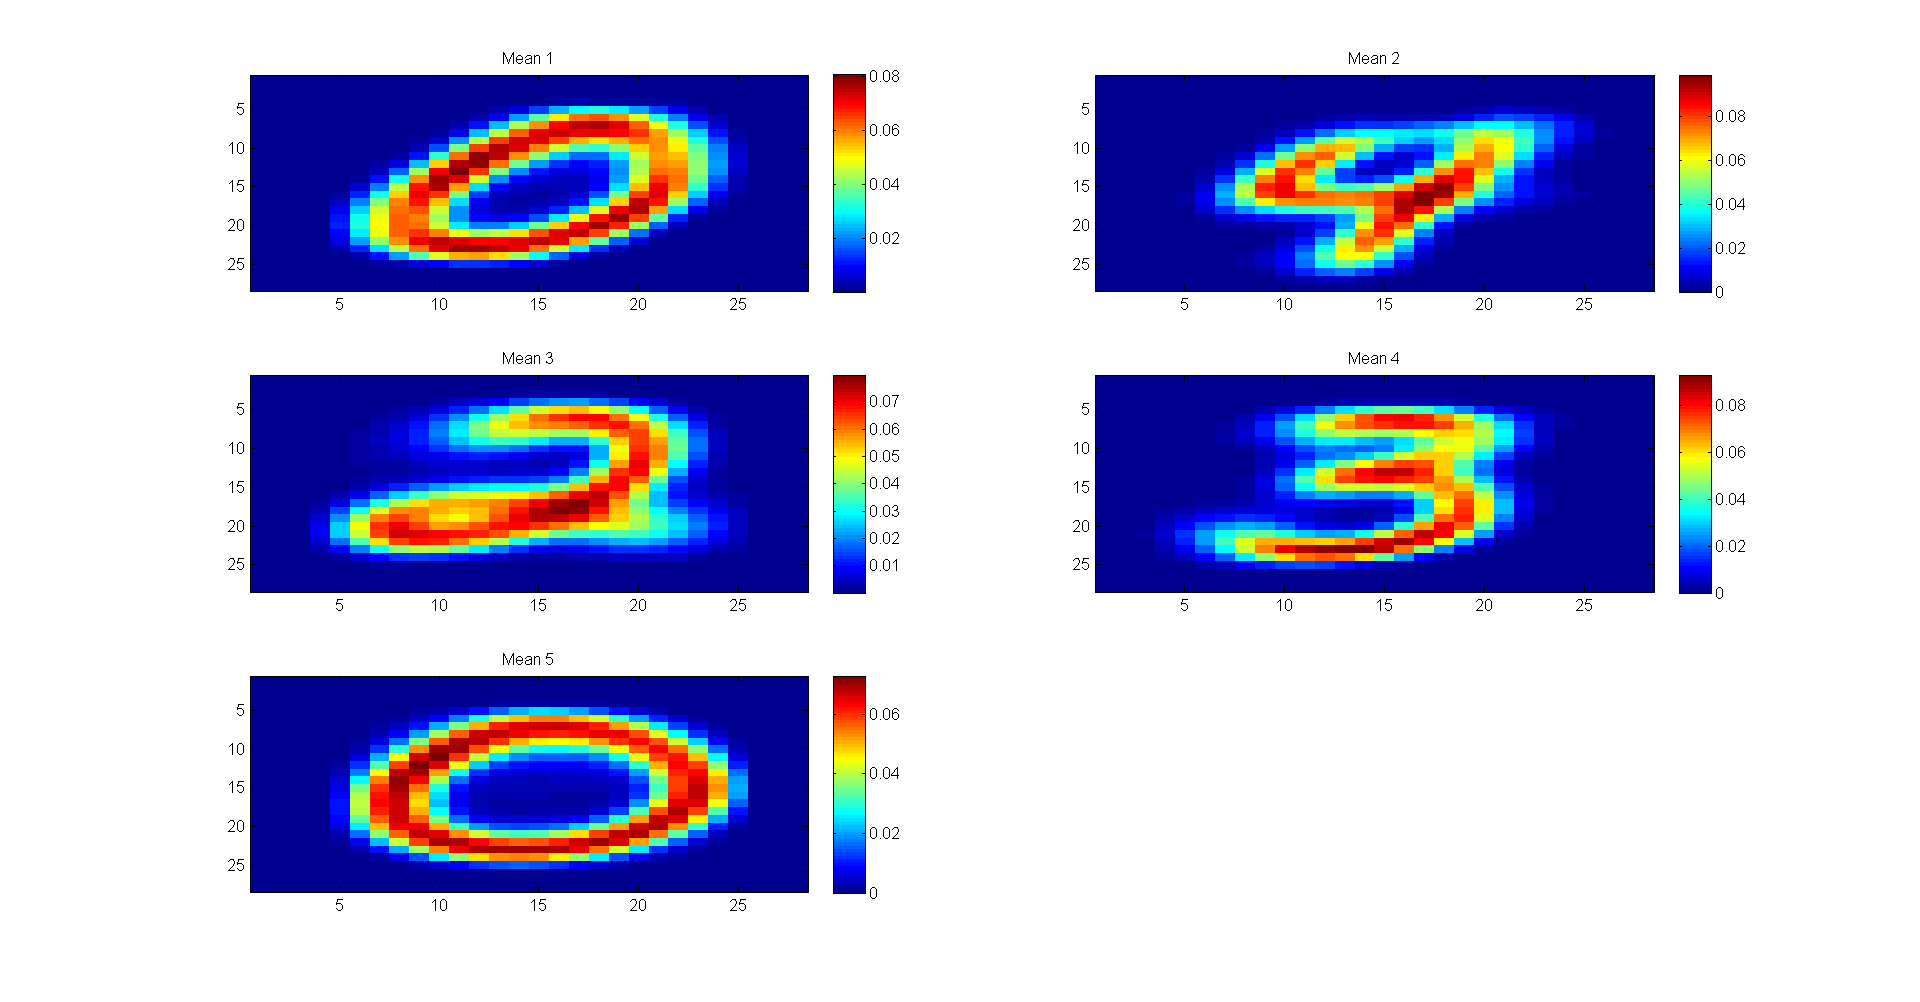
\includegraphics[width=180mm]{images/mean20-1.png}
\label{overflow}
\end{figure}
\begin{figure}[ht!]
\centering
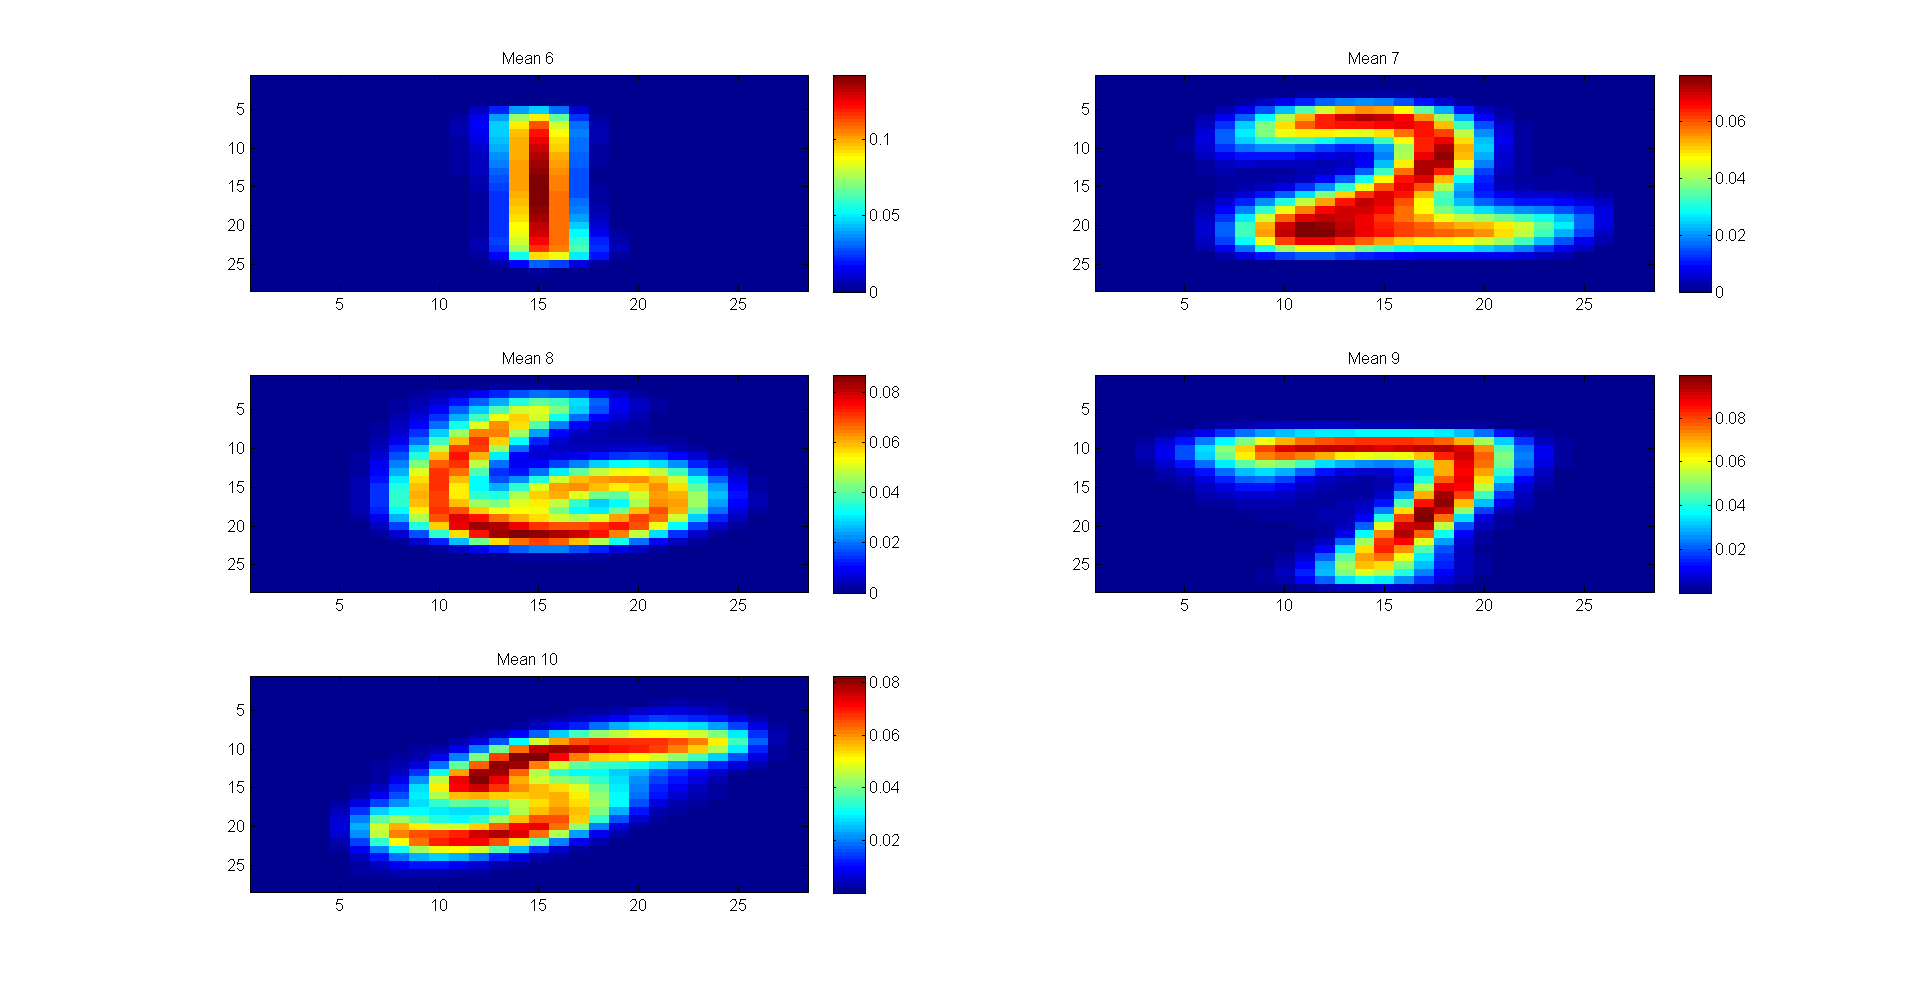
\includegraphics[width=180mm]{images/mean20-2.png}
\label{overflow}
\end{figure}
\newpage
\section*{1. K-Means Clustering on MNIST (page 4 out of 4)}
c) $k=20$ (continued):
\begin{figure}[ht!]
\centering
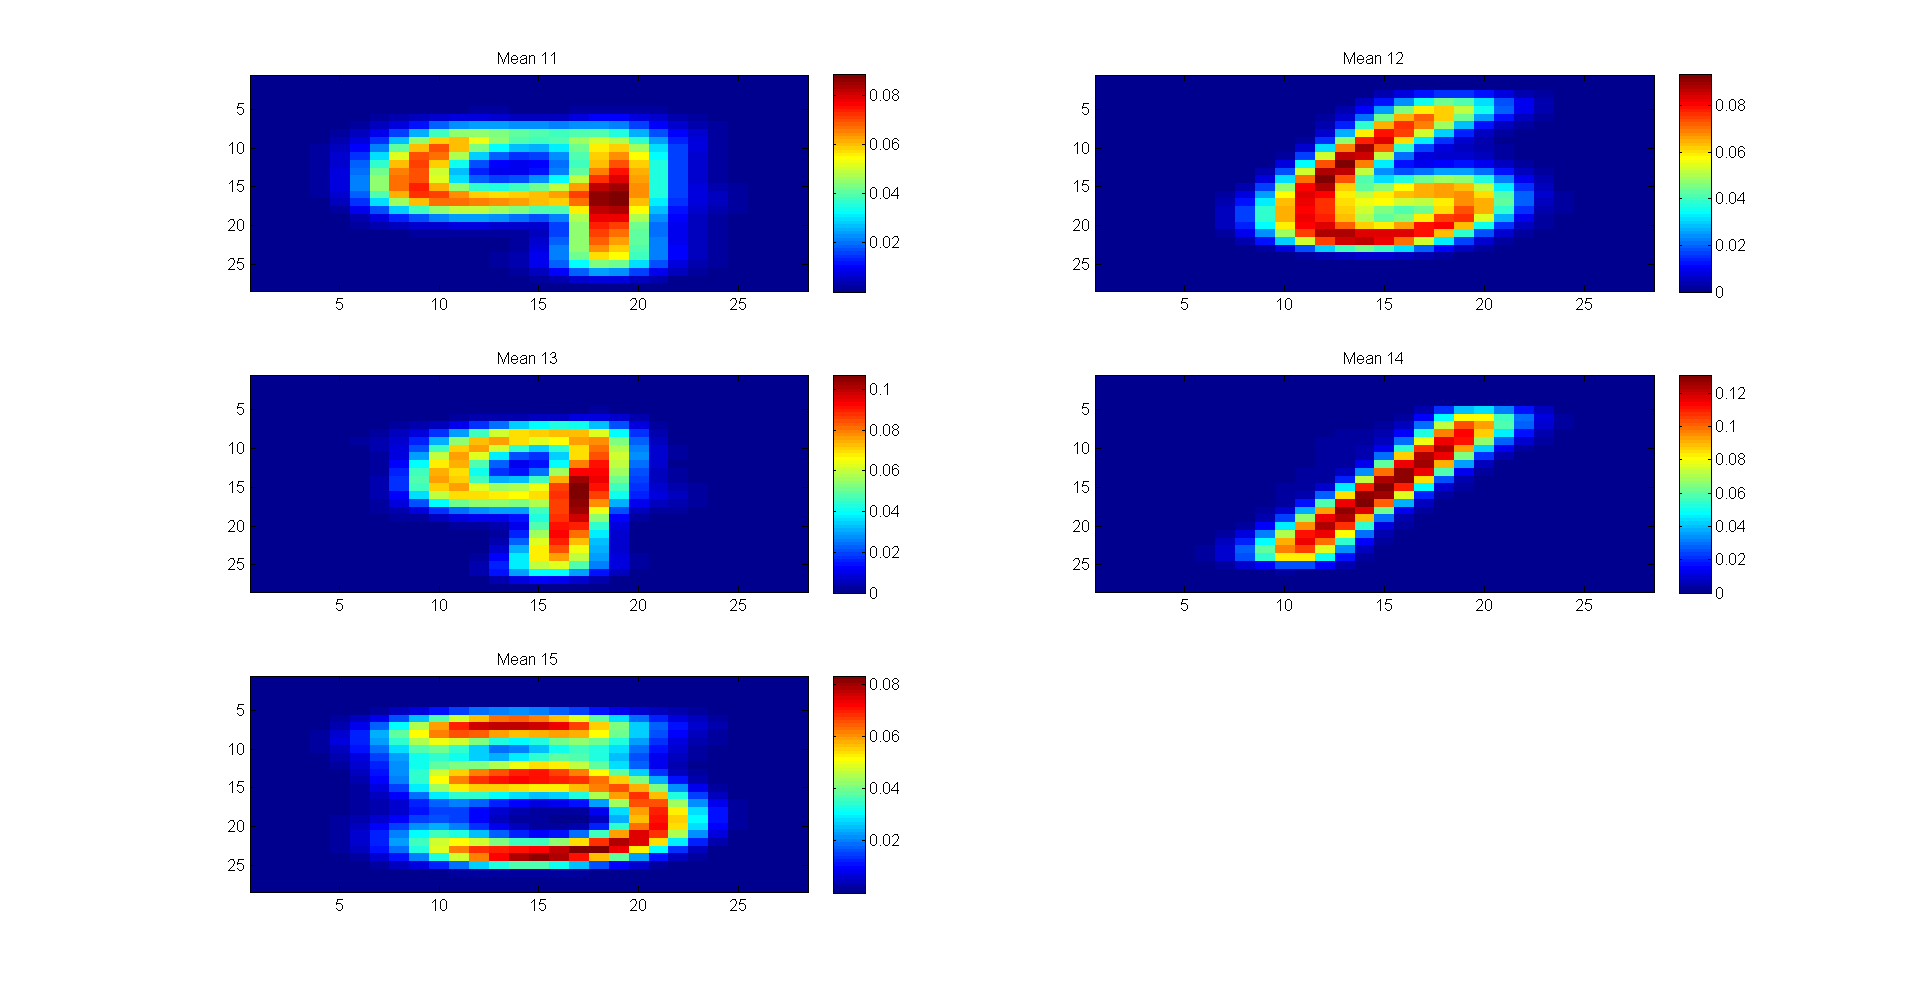
\includegraphics[width=180mm]{images/mean20-3.png}
\label{overflow}
\end{figure}
\begin{figure}[ht!]
\centering
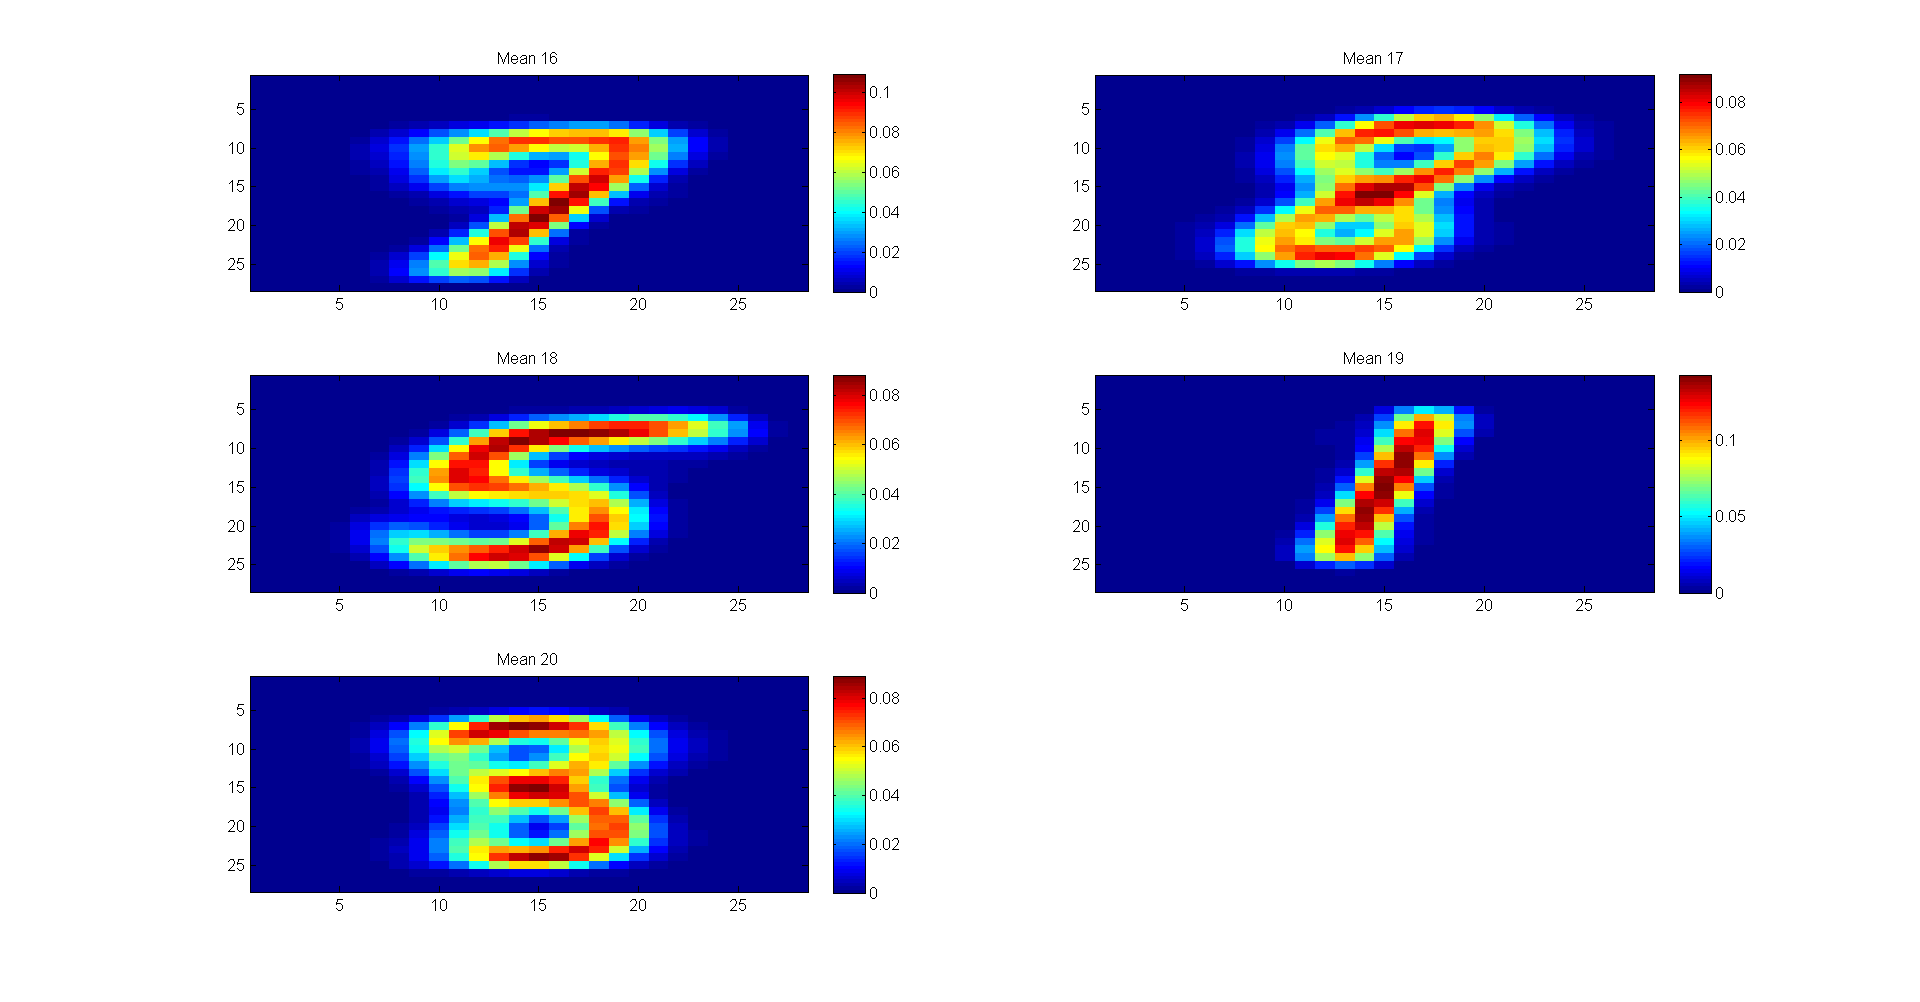
\includegraphics[width=180mm]{images/mean20-4.png}
\label{overflow}
\end{figure}
\newpage

\section*{3. SVD Practice (page 1 out of 4)}
a) $ A = \begin{bmatrix}
2 & 2 \\
1 & -1 \\
\end{bmatrix} $ \\\\
\textbf{(1) Compute $U$ by calculating eigenvectors of $AA^T$.}
\\\\
$AA^T = \begin{bmatrix}
2 & 2 \\
1 & -1 \\
\end{bmatrix} \begin{bmatrix}
2 & 1 \\
2 & -1 \\
\end{bmatrix} = \begin{bmatrix}
8 & 0 \\
0 & 2 \\
\end{bmatrix} $ \\\\
The eigenvalues of $AA^T$ will satisfy $det(A - \lambda I ) = 0$. First, let's compute $A - \lambda I$: \\\\
$ A - \lambda I = \begin{bmatrix}
8 & 0 \\
0 & 2 \\
\end{bmatrix} - \begin{bmatrix}
\lambda & 0 \\
0 & \lambda \\
\end{bmatrix} = \begin{bmatrix}
8 - \lambda & 0 \\
0 & 2 - \lambda \\
\end{bmatrix}$ \\\\
$det(A - \lambda I) = (8 - \lambda) (2 - \lambda)$. \\
Setting the determinant equal to 0 and solving for $\lambda$, we get: $\lambda = 2, 8.$ \\\\
Now we have to find the associated eigenvectors for each eigenvalue. Particularly, we're looking for a $v$ such that $Av = \lambda v$, or, in other words, $(A - \lambda I)v = 0$. \\\\
Let $\lambda = 2$, then $(A - \lambda I) = \begin{bmatrix}
8 - \lambda & 0 \\
0 & 2 - \lambda \\
\end{bmatrix} = \begin{bmatrix}
6 & 0 \\
0 & 0 \\
\end{bmatrix}$. \\\\
Letting $(A - \lambda I)v = 0$, we get that $ \begin{bmatrix}
6 & 0 \\
0 & 0 \\
\end{bmatrix} \begin{bmatrix}
v_0 \\
v_1 \\
\end{bmatrix} = \begin{bmatrix}
6v_0 \\
0 \\
\end{bmatrix} = \begin{bmatrix}
0 \\
0 \\
\end{bmatrix} $. \\\\
For this equality to hold, $v_0$ must be 0. We want the vector to be orthonormal, so set $v_1 = 1$. \\\\
Then: $v = \begin{bmatrix}
0 \\
1 \\
\end{bmatrix}$ is an eigenvector for eigenvalue $\lambda = 2$. \\\\
Let $\lambda = 8$, then $(A - \lambda I) = \begin{bmatrix}
8 - \lambda & 0 \\
0 & 2 - \lambda \\
\end{bmatrix} = \begin{bmatrix}
0 & 0 \\
0 & -6 \\
\end{bmatrix}$. \\\\
Letting $(A - \lambda I)v = 0$, we get that $ \begin{bmatrix}
0 & 0 \\
0 & -6 \\
\end{bmatrix} \begin{bmatrix}
v_0 \\
v_1 \\
\end{bmatrix} = \begin{bmatrix}
0 \\
-6v_1 \\
\end{bmatrix} = \begin{bmatrix}
0 \\
0 \\
\end{bmatrix} $. \\\\
For this equality to hold, $v_1$ must be 0. We want the vector to be orthonormal, so set $v_0 =1$. \\\\
Then: $v = \begin{bmatrix}
1 \\
0 \\
\end{bmatrix}$ is an eigenvector for eigenvalue $\lambda = 8$. \\\\
We'll define $U$ as a 2x2 matrix, where each column contains the corresponding eigenvalues we found:
Hence:
$$ \boxed{ U = \begin{bmatrix} 
v_{\lambda = 2} & v_{\lambda = 8} \\
\end{bmatrix} = \begin{bmatrix}
0 & 1 \\
1 & 0 \\
\end{bmatrix}}$$
\textbf{(2) Compute the entries of $\Sigma$ by calculating the positive square roots of the eigenvalues of $AA^T$.}
\\\\
Since we found the eigenvalues in part (1), we just take the square roots of them and place them in the diagonal matrix corresponding to the order of the eigenvectors in $U$.
$$\boxed{\Sigma = diag(\sqrt2, \sqrt8) = \begin{bmatrix}
\sqrt2 & 0 \\
0 & 2 \sqrt2 \\
\end{bmatrix}} $$

\newpage

\section*{3. SVD Practice (page 2 out of 4)}
\textbf{(3) Compute $V$ by calculating eigenvectors of $A^TA$.}
\\\\
$A^T A= \begin{bmatrix}
2 & 1 \\
2 & -1 \\
\end{bmatrix} \begin{bmatrix}
2 & 2 \\
1 & -1 \\
\end{bmatrix} = \begin{bmatrix}
5 & 3 \\
3 & 5 \\
\end{bmatrix} $ \\\\
The eigenvalues of $AA^T$ will satisfy $det(A - \lambda I ) = 0$. First, let's compute $A - \lambda I$: \\\\
$ A - \lambda I = \begin{bmatrix}
5 & 3 \\
3 & 5 \\
\end{bmatrix} - \begin{bmatrix}
\lambda & 0 \\
0 & \lambda \\
\end{bmatrix} = \begin{bmatrix}
5 - \lambda & 3 \\
3 & 5 - \lambda \\
\end{bmatrix}$ \\\\
$det(A - \lambda I) = (5 - \lambda)^2 - 9 = \lambda^2 - 10\lambda + 16 = (\lambda - 8)(\lambda - 2)$. \\
Setting the determinant equal to 0 and solving for $\lambda$, we get: $\lambda = 2, 8.$ \\\\
Now we have to find the associated eigenvectors for each eigenvalue. Particularly, we're looking for a $v$ such that $Av = \lambda v$, or, in other words, $(A - \lambda I)v = 0$. \\\\
Let $\lambda = 2$, then $(A - \lambda I) = \begin{bmatrix}
5 - \lambda & 3 \\
3 & 5 - \lambda \\
\end{bmatrix} = \begin{bmatrix}
3 & 3 \\
3 & 3 \\
\end{bmatrix}$. \\\\
Letting $(A - \lambda I)v = 0$, we get that $ \begin{bmatrix}
3 & 3 \\
3 & 3 \\
\end{bmatrix} \begin{bmatrix}
v_0 \\
v_1 \\
\end{bmatrix} = \begin{bmatrix}
3v_0 + 3v_1 \\
3v_0 + 3v_1 \\
\end{bmatrix} = \begin{bmatrix}
0 \\
0 \\
\end{bmatrix} $. \\\\
For this equality to hold, $v_0 = -v_1$. We want the vector to be orthonormal, so set $v_0 = 1 / \sqrt2$ and $v_1 = - 1 / \sqrt2.$ \\\\
Then: $v = \begin{bmatrix}
1 / \sqrt2 \\
- 1 / \sqrt2 \\
\end{bmatrix}$ is an eigenvector for eigenvalue $\lambda = 2$. \\\\
Let $\lambda = 8$, then $(A - \lambda I) = \begin{bmatrix}
5 - \lambda & 3 \\
3 & 5 - \lambda \\
\end{bmatrix} = \begin{bmatrix}
-3 & 3 \\
3 & -3 \\
\end{bmatrix}$. \\\\
Letting $(A - \lambda I)v = 0$, we get that $ \begin{bmatrix}
-3 & 3 \\
3 & -3 \\
\end{bmatrix} \begin{bmatrix}
v_0 \\
v_1 \\
\end{bmatrix} = \begin{bmatrix}
-3v_0 + 3v_1 \\
3v_0 -3v_1 \\
\end{bmatrix} = \begin{bmatrix}
0 \\
0 \\
\end{bmatrix} $. \\\\
For this equality to hold, $v_0 = v_1$. We want the vector to be orthonormal, so set $v_0 = 1 / \sqrt2$ and $v_1 = 1 / \sqrt2.$ \\\\
Then: $v = \begin{bmatrix}
1 / \sqrt2 \\
1 / \sqrt2 \\
\end{bmatrix}$ is an eigenvector for eigenvalue $\lambda = 8$. \\\\
We'll define $V$ as a 2x2 matrix, where each column contains the corresponding eigenvalues we found:
Hence:
$$ \boxed{ V = \begin{bmatrix} 
v_{\lambda = 2} & v_{\lambda = 8} \\
\end{bmatrix} = \begin{bmatrix}
1 / \sqrt2 & 1 / \sqrt2 \\
-1 / \sqrt2 & 1 / \sqrt2 \\
\end{bmatrix}}$$
\textbf{(4) Verify that $A = U \Sigma V^T.$}
$$\begin{aligned}
U \Sigma V^T &= \begin{bmatrix}
0 & 1 \\
1 & 0 \\
\end{bmatrix} \begin{bmatrix}
\sqrt2 & 0 \\
0 & 2 \sqrt2 \\
\end{bmatrix} \begin{bmatrix}
1 / \sqrt2 & -1 / \sqrt2 \\
1 / \sqrt2 & 1 / \sqrt2 \\
\end{bmatrix} \\
&= \begin{bmatrix}
0 & 2 \sqrt2 \\
\sqrt2 & 0 \\
\end{bmatrix} \begin{bmatrix}
1 / \sqrt2 & -1 / \sqrt2 \\
1 / \sqrt2 & 1 / \sqrt2 \\
\end{bmatrix} \\
&= \begin{bmatrix}
2 & 2 \\
1 & -1 \\
\end{bmatrix} \\
&= \boxed{A}
\end{aligned} $$


\section*{3. SVD Practice (page 3 out of 4)}
a) $ A = \begin{bmatrix}
2 & 2 \\
1 & 1 \\
\end{bmatrix} $ \\\\
\textbf{(1) Compute $U$ by calculating eigenvectors of $AA^T$.}
\\\\
$AA^T = \begin{bmatrix}
2 & 2 \\
1 & 1 \\
\end{bmatrix} \begin{bmatrix}
2 & 1 \\
2 & 1 \\
\end{bmatrix} = \begin{bmatrix}
8 & 4 \\
4 & 2 \\
\end{bmatrix} $ \\\\
The eigenvalues of $AA^T$ will satisfy $det(A - \lambda I ) = 0$. First, let's compute $A - \lambda I$: \\\\
$ A - \lambda I = \begin{bmatrix}
8 & 4 \\
4 & 2 \\
\end{bmatrix} - \begin{bmatrix}
\lambda & 0 \\
0 & \lambda \\
\end{bmatrix} = \begin{bmatrix}
8 - \lambda & 4 \\
4 & 2 - \lambda \\
\end{bmatrix}$ \\\\
$det(A - \lambda I) = (8 - \lambda) (2 - \lambda) - 16 = \lambda^2 - 10\lambda + 16 - 16 = \lambda (\lambda - 10)$. \\
Setting the determinant equal to 0 and solving for $\lambda$, we get: $\lambda = 0, 10.$ \\\\
Now we have to find the associated eigenvectors for each eigenvalue. Particularly, we're looking for a $v$ such that $Av = \lambda v$, or, in other words, $(A - \lambda I)v = 0$. \\\\
Let $\lambda = 0$, then $(A - \lambda I) = \begin{bmatrix}
8 - \lambda & 4 \\
4 & 2 - \lambda \\
\end{bmatrix} = \begin{bmatrix}
8 & 4 \\
4 & 2 \\
\end{bmatrix}$. \\\\
Letting $(A - \lambda I)v = 0$, we get that $ \begin{bmatrix}
8 & 4 \\
4 & 2 \\
\end{bmatrix} \begin{bmatrix}
v_0 \\
v_1 \\
\end{bmatrix} = \begin{bmatrix}
8v_0 + 4v_1 \\
4v_0 + 2v_1 \\
\end{bmatrix} = \begin{bmatrix}
0 \\
0 \\
\end{bmatrix} $. \\\\
For this equality to hold, $-2v_0 = v_1$. We want the vector to be orthonormal, so set $v_0 = 1 / \sqrt5$ and $v_1 = - 2 / \sqrt5.$ \\\\
Then: $v = \begin{bmatrix}
1 / \sqrt5 \\
-2 / \sqrt5 \\
\end{bmatrix}$ is an eigenvector for eigenvalue $\lambda = 0$. \\\\
Let $\lambda = 10$, then $(A - \lambda I) = \begin{bmatrix}
8 - \lambda & 4 \\
4 & 2 - \lambda \\
\end{bmatrix} = \begin{bmatrix}
-2 & 4 \\
4 & -8 \\
\end{bmatrix}$. \\\\
Letting $(A - \lambda I)v = 0$, we get that $ \begin{bmatrix}
-2 & 4 \\
4 & -8 \\
\end{bmatrix} \begin{bmatrix}
v_0 \\
v_1 \\
\end{bmatrix} = \begin{bmatrix}
-2v_0 + 4v_1 \\
4v_0 - 8v_1 \\
\end{bmatrix} = \begin{bmatrix}
0 \\
0 \\
\end{bmatrix} $. \\\\
For this equality to hold, $v_0 = 2v_1$. We want the vector to be orthonormal, so set $v_0 = 2 / \sqrt5$ and $v_1 = 1 / \sqrt5.$ \\\\
Then: $v = \begin{bmatrix}
2 / \sqrt5 \\
1 / \sqrt5 \\
\end{bmatrix}$ is an eigenvector for eigenvalue $\lambda = 10$. \\\\
We'll define $U$ as a 2x2 matrix, where each column contains the corresponding eigenvalues we found:
Hence:
$$ \boxed{ U = \begin{bmatrix} 
v_{\lambda = 0} & v_{\lambda = 10} \\
\end{bmatrix} = \begin{bmatrix}
1 / \sqrt5 & 2 / \sqrt5 \\
-2 / \sqrt5 & 1 / \sqrt5 \\
\end{bmatrix}}$$
\textbf{(2) Compute the entries of $\Sigma$ by calculating the positive square roots of the eigenvalues of $AA^T$.}
\\\\
Since we found the eigenvalues in part (1), we just take the square roots of them and place them in the diagonal matrix corresponding to the order of the eigenvectors in $U$.
$$\boxed{\Sigma = diag(0, \sqrt{10}) = \begin{bmatrix}
0 & 0 \\
0 & \sqrt{10} \\
\end{bmatrix}} $$

\newpage

\section*{3. SVD Practice (page 4 out of 4)}
\textbf{(3) Compute $V$ by calculating eigenvectors of $A^TA$.}
\\\\
$A^T A= \begin{bmatrix}
2 & 1 \\
2 & 1 \\
\end{bmatrix} \begin{bmatrix}
2 & 2 \\
1 & 1 \\
\end{bmatrix} = \begin{bmatrix}
5 & 5 \\
5 & 5 \\
\end{bmatrix} $ \\\\
The eigenvalues of $AA^T$ will satisfy $det(A - \lambda I ) = 0$. First, let's compute $A - \lambda I$: \\\\
$ A - \lambda I = \begin{bmatrix}
5 & 5 \\
5 & 5 \\
\end{bmatrix} - \begin{bmatrix}
\lambda & 0 \\
0 & \lambda \\
\end{bmatrix} = \begin{bmatrix}
5 - \lambda & 5 \\
5 & 5 - \lambda \\
\end{bmatrix}$ \\\\
$det(A - \lambda I) = (5 - \lambda)^2 - 25 = \lambda^2 - 10\lambda + 25 - 25 = \lambda(\lambda - 10)$. \\
Setting the determinant equal to 0 and solving for $\lambda$, we get: $\lambda = 0, 10.$ \\\\
Now we have to find the associated eigenvectors for each eigenvalue. Particularly, we're looking for a $v$ such that $Av = \lambda v$, or, in other words, $(A - \lambda I)v = 0$. \\\\
Let $\lambda = 0$, then $(A - \lambda I) = \begin{bmatrix}
5 - \lambda & 5 \\
5 & 5 - \lambda \\
\end{bmatrix} = \begin{bmatrix}
5 & 5 \\
5 & 5 \\
\end{bmatrix}$. \\\\
Letting $(A - \lambda I)v = 0$, we get that $ \begin{bmatrix}
5 & 5 \\
5 & 5 \\
\end{bmatrix} \begin{bmatrix}
v_0 \\
v_1 \\
\end{bmatrix} = \begin{bmatrix}
5v_0 + 5v_1 \\
5v_0 + 5v_1 \\
\end{bmatrix} = \begin{bmatrix}
0 \\
0 \\
\end{bmatrix} $. \\\\
For this inequality to hold, $v_0 = -v_1$. We want the vector to be orthonormal, so set $v_0 = 1 / \sqrt2$ and $v_1 = - 1 / \sqrt2.$ \\\\
Then: $v = \begin{bmatrix}
1 / \sqrt2 \\
- 1 / \sqrt2 \\
\end{bmatrix}$ is an eigenvector for eigenvalue $\lambda = 0$. \\\\
Let $\lambda = 10$, then $(A - \lambda I) = \begin{bmatrix}
5 - \lambda & 5 \\
5 & 5 - \lambda \\
\end{bmatrix} = \begin{bmatrix}
-5 & 5 \\
5 & -5 \\
\end{bmatrix}$. \\\\
Letting $(A - \lambda I)v = 0$, we get that $ \begin{bmatrix}
-5 & 5 \\
5 & -5 \\
\end{bmatrix} \begin{bmatrix}
v_0 \\
v_1 \\
\end{bmatrix} = \begin{bmatrix}
-5v_0 + 5v_1 \\
5v_0 -5v_1 \\
\end{bmatrix} = \begin{bmatrix}
0 \\
0 \\
\end{bmatrix} $. \\\\
For this inequality to hold, $v_0 = v_1$. We want the vector to be orthonormal, so set $v_0 = 1 / \sqrt2$ and $v_1 = 1 / \sqrt2.$ \\\\
Then: $v = \begin{bmatrix}
1 / \sqrt2 \\
1 / \sqrt2 \\
\end{bmatrix}$ is an eigenvector for eigenvalue $\lambda = 10$. \\\\
We'll define $V$ as a 2x2 matrix, where each column contains the corresponding eigenvalues we found:
Hence:
$$ \boxed{ V = \begin{bmatrix} 
v_{\lambda = 0} & v_{\lambda = 10} \\
\end{bmatrix} = \begin{bmatrix}
1 / \sqrt2 & 1 / \sqrt2 \\
-1 / \sqrt2 & 1 / \sqrt2 \\
\end{bmatrix}}$$
\textbf{(4) Verify that $A = U \Sigma V^T.$}
$$\begin{aligned}
U \Sigma V^T &=\begin{bmatrix}
1 / \sqrt5 & 2 / \sqrt5 \\
-2 / \sqrt5 & 1 / \sqrt5 \\
\end{bmatrix} \begin{bmatrix}
0 & 0 \\
0 & \sqrt{10} \\
\end{bmatrix} \begin{bmatrix}
1 / \sqrt2 & -1 / \sqrt2 \\
1 / \sqrt2 & 1 / \sqrt2 \\
\end{bmatrix} \\
&= \begin{bmatrix}
0 & 2 \sqrt2 \\
0 & \sqrt2 \\
\end{bmatrix} \begin{bmatrix}
1 / \sqrt2 & -1 / \sqrt2 \\
1 / \sqrt2 & 1 / \sqrt2 \\
\end{bmatrix} \\
&= \begin{bmatrix}
2 & 2 \\
1 & 1 \\
\end{bmatrix} \\
&= \boxed{A}
\end{aligned} $$

\end{document}